% !TEX root = main.tex

%%%%%%%%%%%%%%%%%%%%%%%%%%%%%%%%%%%%%%%%%%%%%%%%%%%%%%%%%%%%
\appendices

\section{Definition of the derivatives in $SO(3)$}
\label{sec:derivatives_SO3}

\subsection{The additive and subtractive operators in $SO(3)$}

\begin{figure}[tb]
\begin{center}
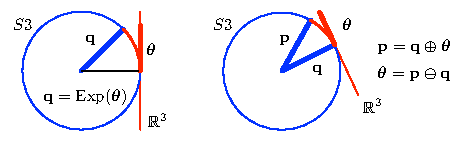
\includegraphics{figures/manifold}
\caption{The S3 manifold is a unit sphere in $\bbR^4$, here represented by a unit circle (blue),  where all unit quaternions live. The tangent space at the element $\bfq$ is the hyperplane $\bbR^3$, here represented by a line (red). The $\oplus$ and $\ominus$ operators relate elements of the manifold with elements in the tangent space. The analogy may serve to illustrate also the $SO(3)$ manifold.}
\label{fig:manifold}
\end{center}
\end{figure}



\paragraph{The plus operator.}
The `plus' operator $\oplus:SO(3)\times\bbR^3\to SO(3)$ (\figRef{fig:manifold}) produces an element $\sS$ of $SO(3)$ which is the result of composing a reference element $\sR$ of $SO(3)$ with a (often small) rotation specified by a vector of $\bth\in\bbR^3$ that is tangent to the $SO(3)$ manifold at the reference element $\sR$,
%
\begin{align}
\sS = \sR\oplus \bth &\te \sR\circ\Exp(\bth) && \sR,\sS\in SO(3),~ \bth\in\bbR^3 
\end{align}
%
Notice that this operator may be defined for any representation of $SO(3)$. In particular, 
%
\begin{align}
\bfq\oplus\bth &= \bfq\ot\Exp(\bth) \\
\bfR\oplus \bth &= \bfR\Exp(\bth) 
\end{align}

\paragraph{The minus operator.}
The `minus' operator $\ominus:SO(3)\times SO(3)\to\bbR^3$ (\figRef{fig:manifold}) is the inverse of the above,
%. It returns the  angular difference vector $\bth\in\bbR^3$ between two elements of $SO(3)$. This vector is tangent to the $SO(3)$ manifold at the reference element $\sR$, 
%
\begin{align}
\bth=\sS\ominus \sR
&\te \Log(\sR\inv \circ \sS)     && \sR,\sS\in SO(3),~ \bth\in\bbR^3  
\end{align}
%
and in particular,
%
\begin{align}
\bth &= \bfq\ominus\bfp = \Log(\bfp^*\ot\bfq)                      \\
\bth &= \bfS\ominus\bfR = \Log(\bfR\tr\,\bfS)                         
\end{align}



\subsection{The four possible derivative definitions}

\subsubsection{Functions from vector space to vector space}

We use the standard operators $\{+,-\}$ to define the derivative as
%
\begin{align}
\dpar{f(\bfx)}{\bfx} &\te \lim_{\delta\bfx\to0}\frac{f(\bfx+\delta\bfx)-f(\bfx)}{\delta\bfx} &&\in \bbR^{n\times m} \label{equ:derivative_vector}
\end{align}

\subsubsection{Functions from $SO(3)$ to $SO(3)$}

We use the $SO(3)$ operators $\{\oplus,\ominus\}$ to define the derivative as
%
\begin{align}
\dpar{f(\sR)}{\bth} 
&\te \lim_{\delta\bth\to0}\frac{f(\sR\oplus\delta\bth)\ominus f(\sR)}{\delta\bth}  && \in \bbR^{3\times 3}
\label{equ:derivative_SO3}
\end{align}

\subsubsection{Functions from vector space to $SO(3)$}

We use `+' for the vector perturbations, and `$\ominus$' for the $SO(3)$ difference,
%
\begin{align}
\dpar{f(\bfx)}{\bfx} &\te \lim_{\delta\bfx\to0} \frac{ f(\bfx+\delta\bfx)\ominus f(\bfx)}{\delta\bfx} && \in \bbR^{3\times m} \label{equ:dif_RtoSO3}
\end{align}


\subsubsection{Functions from $SO(3)$ to vector space}


We use `$\oplus$' for the $SO(3)$ perturbations, and `$-$' for the vector difference,
%
\begin{align}
\dpar{f(\sR)}{\bth} &\te \lim_{\delta\bth\to0} \frac{f(\sR\oplus\delta\bth) - f(\sR)}{\delta\bth} && \in \bbR^{n\times 3} \label{equ:jacobian_SO3_Rn}
\end{align}



\subsection{Right Jacobian of $SO(3)$ }

We define the right Jacobian of $SO(3)$ as, 
%
\begin{align}
\bfJ_r(\bth) &\te \dpar{\Exp(\bth)}{\bth} 
\end{align}
%
Since the exponential $\Exp()$ is an application $\bbR^3\to SO(3)$,
we implement this derivative using \eqRef{equ:dif_RtoSO3}.
The right Jacobian and its inverse can be computed in closed form with
%
\begin{align}
\bfJ_r(\bth) &= \bfI - \frac{1-\cos\nth}{\nth^2}\hatx{\bth} + \frac{\nth-\sin\nth}{\nth^3}\hatx{\bth}^2 \\
\bfJ_r\inv(\bth) &= \bfI + \frac12\hatx{\bth} + \left(\frac1{\nth^2} - \frac{1+\cos\nth}{2\nth\sin\nth}\right)\hatx{\bth}^2
\end{align}






%%%%%%%%%%%%%%%%%%%%%%%%%%%%%%%%%%%%%%%%%%%%%%%%%%%%%%%%%%%%%%%%%%%%%%%%%%%
\subsection{Useful properties for Jacobian development}
\label{sec:DosDonts}

We provide a collection of rules which come very handy to develop Jacobians. They come organized under helper \com{keys}\!\!\!\!, which we use to refer to each of these properties in our developments.


\paragraph{\ccross : Skew-symmetric matrix}
%
\begin{align}
\hatx{\bfa}\bfb &= -\hatx{\bfb}\bfa 
\\
\hatx{\bfR\bfa} &= \bfR\hatx{\bfa}\bfR\tr 
\end{align}

\paragraph{\cJr : Right Jacobian of $SO(3)$ }

It has the properties, for any $\bth$ and small $\dth$,
%
\begin{align}
\Exp(\bth+\dth) &\approx \Exp(\bth)\Exp(\bfJ_r(\bth)\dth) \\
\Exp(\bth)\Exp(\dth) &\approx \Exp(\bth+\bfJ_r\inv(\bth)\,\dth) 
\end{align}
%






\paragraph{\csmall : Small angle approximations}

Let $\dth$ be a small angle vector. Then,
%
\begin{align}
\Exp(\dth) &\approx \bfI + \hatx{\dth} \\
\bfJ_r(\dth) &\approx \bfI - \frac12\hatx{\dth} 
\end{align}



\paragraph{\cexpand, \csubst, \ccancel : Expand, substitute, cancel} This happens when we expand or substitute a previously defined term, or when we cancel terms.



\subsection{Examples}

\subsubsection{Function $SO(3)\times\bbR^3\to SO(3)$} 
\label{sec:jac_R3toSO3}

The function $f(\sR,\bw) = \bfq\od\Exp(\bw\dt) = \bfR\Exp(\bw\dt)\in SO(3)$ produces elements of $SO(3)$ from elements $\sR\in SO(3)$ and vectors $\bw\in\bbR^3$. 
Its Jacobian \wrt $\bw$ is defined by \eqRef{equ:dif_RtoSO3} and develops as,
%
\begin{align*}
\dpar{\bfR\Exp(\bw\dt)}{\bw} 
&= \lim_{\delta\bw\to0}\frac{\bfR\Exp((\bw+\delta\bw)\dt) \ominus (\bfR\Exp(\bw\dt)) }{\delta\bw} \\
\com{$\ominus$}
&= \lim_{\delta\bw\to0}\frac{\Log\big((\bfR\Exp(\bw\dt))\inv \, \bfR\Exp(\bw\dt+\delta\bw\dt)\big)}{\delta\bw} \\
\cJr
&= \lim_{\delta\bw\to0}\frac{\Log\big((\bfR\Exp(\bw\dt))\inv \bfR\Exp(\bw\dt)\Exp(\bfJ_r(\bw\dt)\delta\bw\dt)\big)}{\delta\bw} \\
\ccancel
&= \lim_{\delta\bw\to0}\frac{\Log\big(\Exp(\bfJ_r(\bw\dt)\delta\bw\dt)\big)}{\delta\bw} \\
\com{cancel}
&= \bfJ_r(\bw\dt)\dt
\end{align*}
%


\subsubsection{Function $SO(3)\times\bbR^3\to\bbR^3$} 
\label{sec:jac_SO3xR3toR3}

The rotation $f(\sR,\bfv) = \bfq\od\bfv = \bfR\,\bfv \in \bbR^3$ produces vectors of $\bbR^3$ from elements $\sR\in SO(3)$ and vectors $\bfv\in\bbR^3$. The first Jacobian is defined by \eqRef{equ:jacobian_SO3_Rn} and developed as
%
\begin{align*}
\dpar{\bfq\od\bfv}{\bth} = \dpar{\bfR\bfv}{\bth} 
&\te \lim_{\delta\bth\to0}\frac{(\bfR\oplus\delta\bth)\bfv-\bfR\bfv}{\delta\bth} \\
\com{$\oplus$}
&= \lim_{\delta\bth\to0}\frac{\bfR\Exp(\delta\bth)\bfv-\bfR\bfv}{\delta\bth} \\
\csmall
&= \lim_{\delta\bth\to0}\frac{\bfR\tdot(\bfI+\hatx{\delta\bth})\bfv-\bfR\bfv}{\delta\bth} \\
\ccancel
&= \lim_{\delta\bth\to0}\frac{\bfR\hatx{\delta\bth}\bfv}{\delta\bth} \\
\ccross
&= \lim_{\delta\bth\to0}\frac{-\bfR\hatx{\bfv}\delta\bth}{\delta\bth} \\
&= -\bfR\hatx{\bfv} 
\end{align*}
%
The second  is defined by \eqRef{equ:derivative_vector} and trivially develops as,
%
\begin{align*}
\dpar{\bfq\od\bfv}{\bfv} = \dpar{\bfR\bfv}{\bfv} 
&\te \lim_{\partial\bfv\to0}\frac{\bfR\tdot(\bfv+\partial\bfv)-\bfR\bfv}{\partial\bfv} 
= \bfR
\end{align*}





